\begin{figure}[htp]
	\centering
	\subfloat[\(\mesh{W^{\Phi}}\)]
	{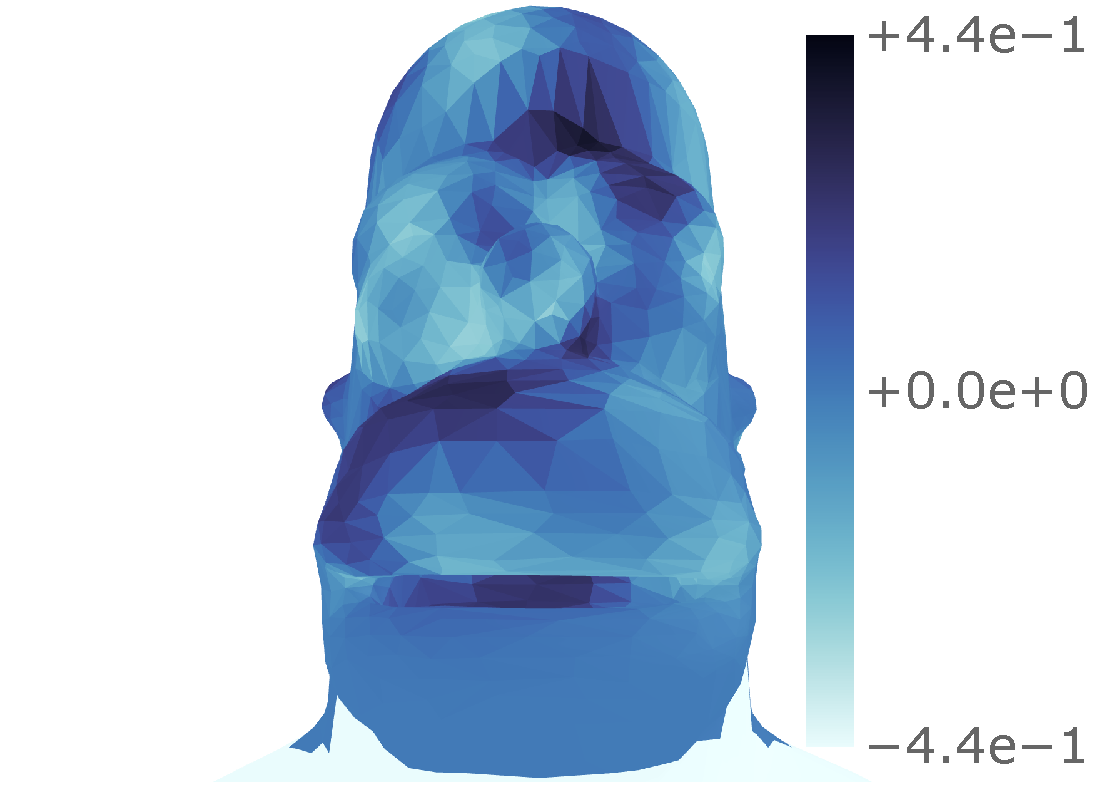
\includegraphics[trim={102 3 6 2},clip,width=.33\textwidth]{chapter4/slepian_wavelet_coefficients_homer_3B_2jmin_scaling_zoom.pdf}}
	\hfill
	\subfloat[\(\mesh{W^{\Psi^{2j}}}\)]
	{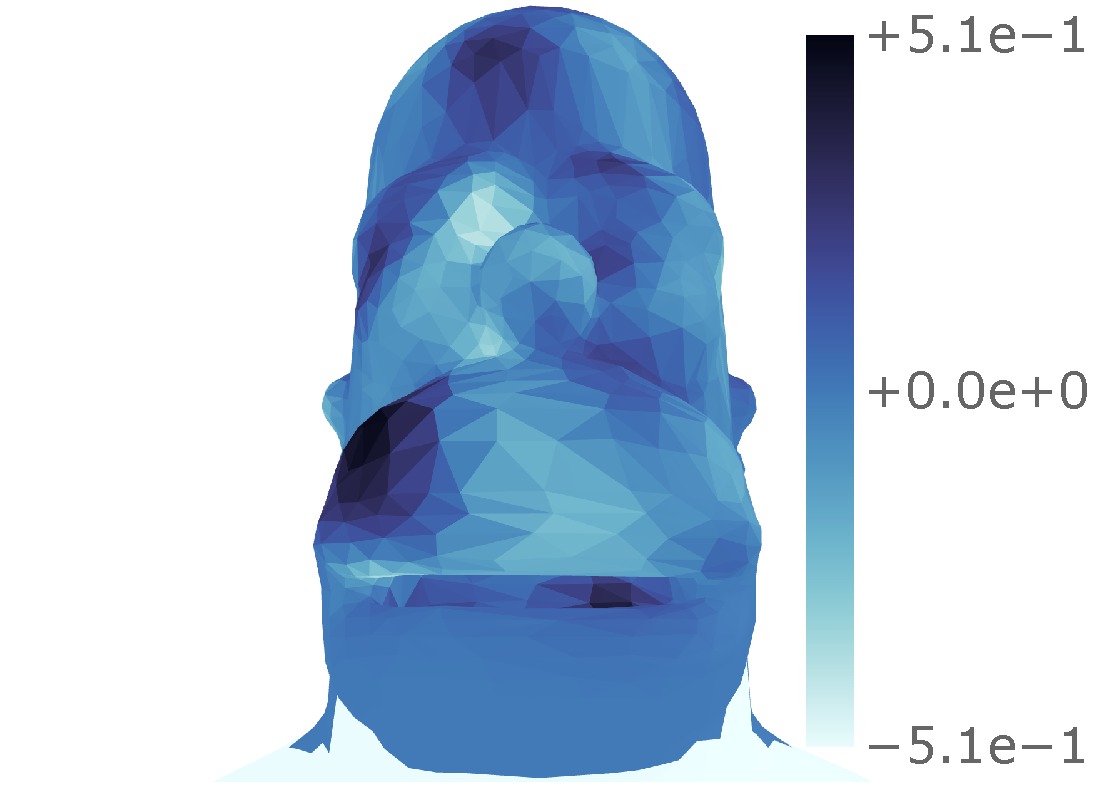
\includegraphics[trim={102 3 6 2},clip,width=.33\textwidth]{chapter4/slepian_wavelet_coefficients_homer_3B_2jmin_2j_zoom.pdf}}
	\hfill
	\subfloat[\(\mesh{W^{\Psi^{3j}}}\)]
	{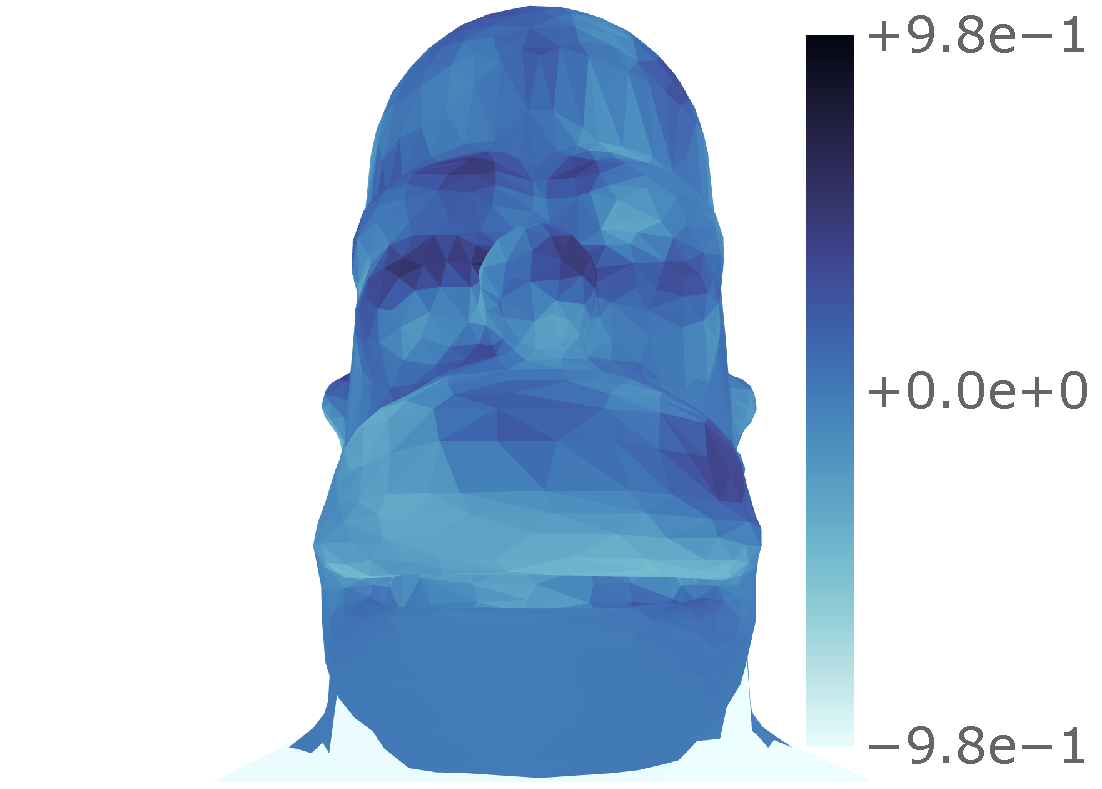
\includegraphics[trim={102 3 6 2},clip,width=.33\textwidth]{chapter4/slepian_wavelet_coefficients_homer_3B_2jmin_3j_zoom.pdf}}
	\newline
	\subfloat[\(\mesh{W^{\Psi^{4j}}}\)]
	{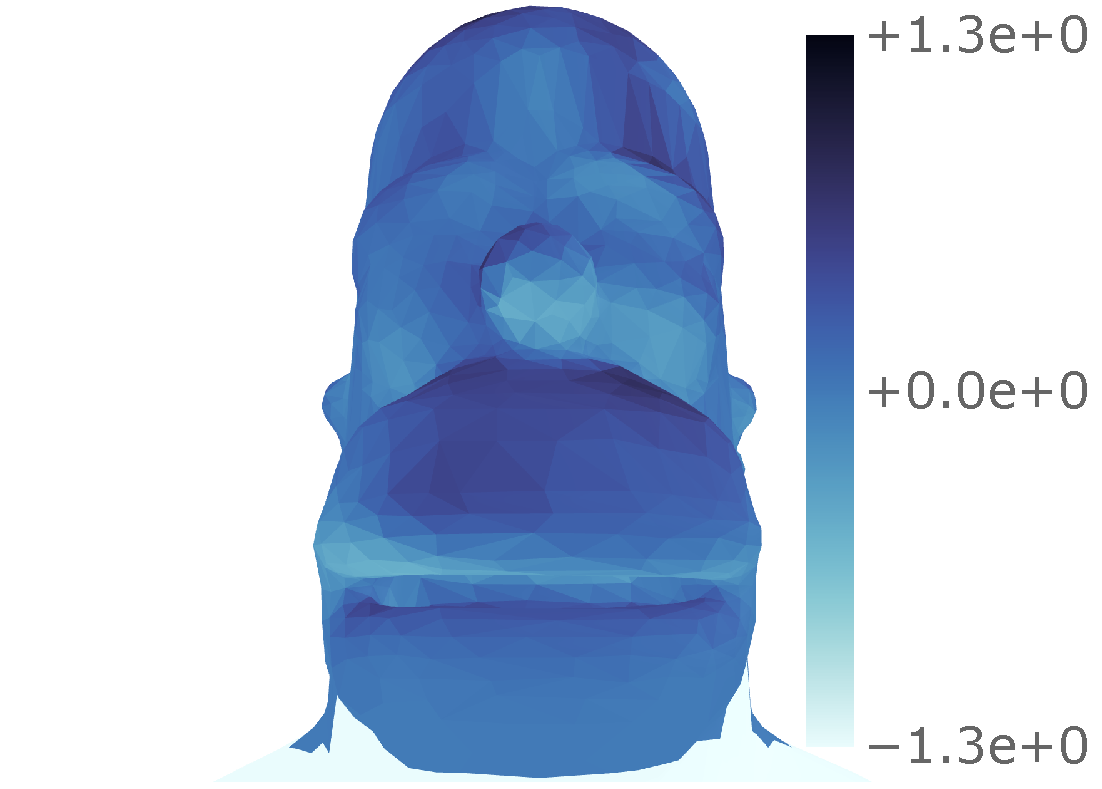
\includegraphics[trim={102 3 6 2},clip,width=.33\textwidth]{chapter4/slepian_wavelet_coefficients_homer_3B_2jmin_4j_zoom.pdf}}
	\hfill
	\subfloat[\(\mesh{W^{\Psi^{5j}}}\)]
	{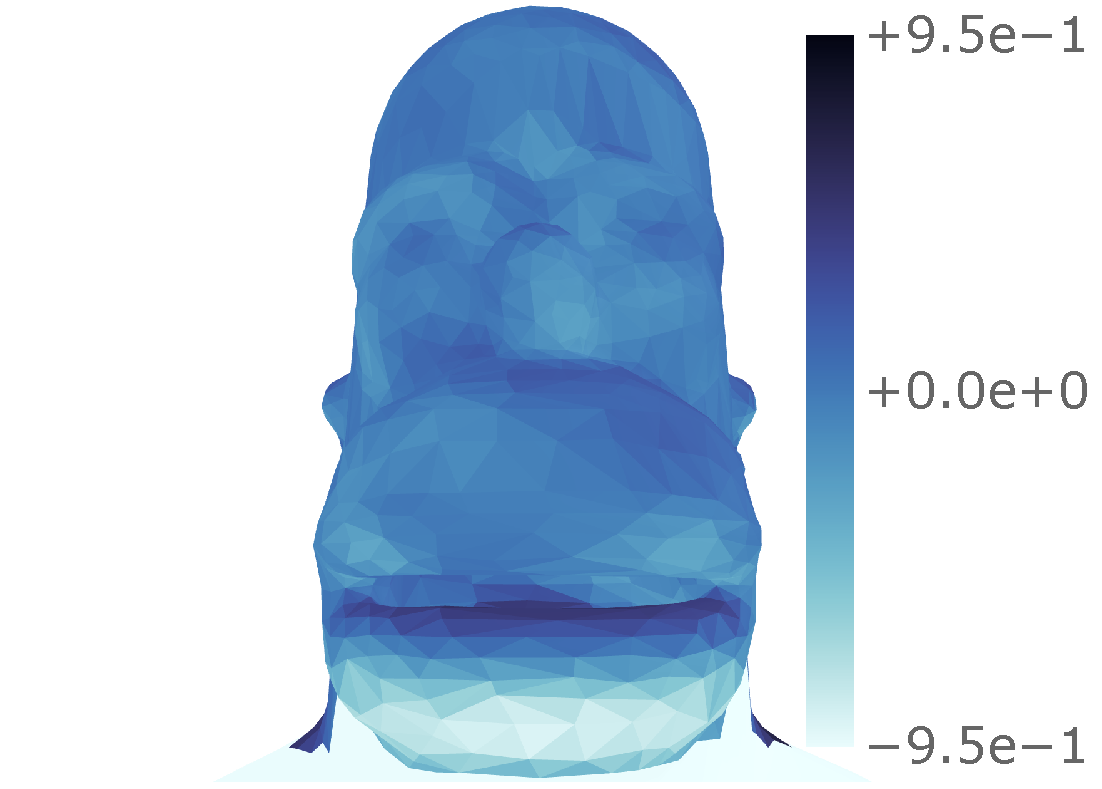
\includegraphics[trim={102 3 6 2},clip,width=.33\textwidth]{chapter4/slepian_wavelet_coefficients_homer_3B_2jmin_5j_zoom.pdf}}
	\hfill
	\subfloat[\(\mesh{W^{\Psi^{6j}}}\)]
	{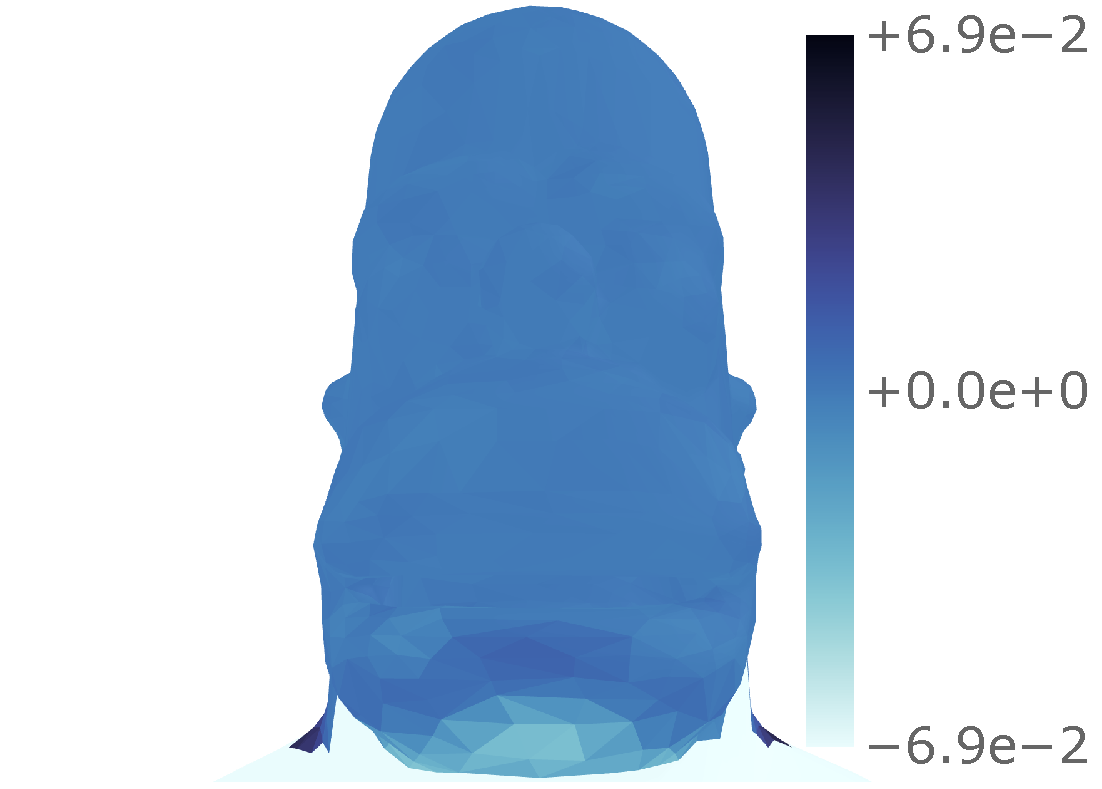
\includegraphics[trim={102 3 6 2},clip,width=.33\textwidth]{chapter4/slepian_wavelet_coefficients_homer_3B_2jmin_6j_zoom.pdf}}
	\caption{
	}\label{fig:chapter4_wavelet_coefficients}
\end{figure}
